\chapter{Implementation}

In this chapter we will take a close look into the overall functioning of an football articles generating NLG system. The goal was to create an end-to-end NLG system, that takes non-processed raw data about a football match as an input and creates article in Czech language that summarises the development of a match. The aim of the thesis was not only to get the basic understanding of a NLG process, but also try to create the implementation in a language that is widely used around the world and for me, personally, was less known - Python.

\section{Requirements and initial goal}
As mentioned in the introduction of this section, the expected output was simply a readable Czech text summary while attempting to produce sentences that are not identical resulting in less-monotonic text. Since the expected output was defined as somewhat vague and quality-wise uncertain, there is no stress on the definition of goal of the language and target audience. However, the text quality, especially in the variability of expressions, used structures and overall richness, is insufficient to truly satisfy the definition of an article. 

Since NLG is a complex process we used one already existing tool for linguistic realisation - \emph{Geneea API}. Without this tool the output language would not be grammatically correct and therefore not satisfying the readability requirement. As discussed in (TODO-A-ref na linguistic realisation) this task has no easy way of implementing manually, especially not for a Czech language that belongs to the most complicated natural languages (for reasons that are described in (TODO-A-ref na linguistic realisation)). \emph{Geneea API} usage skips this task focusing on the rest of the NLG tasks combined.

In \autoref{chap:process} (TODO - A - ref a whole section) We proposed an outline to a requirements analysis. This section will follow this structure describing the specifics.

\section{Input data}
Dataset was provided by a company Livesport s.r.o. (TODO-A-mám ji zmiňovat), which I would like to thank. Therefore entire dataset can not be shared. However, one example match is attached to illustrate program functioning. Initial dataset is composed of every match of one Czech First League season. Every match is represented as JSON file storing both general information about the match (teams, venue, attendance, line-ups, etc.) and course of key events of the matches (goals, substitutions, cards, etc.). 

General information about the match consists of two participating teams, starting time of the match, tournament information (here it is Czech First League for the particular year), information about venue, score, winner, stage of the game (e.g. finished/delayed) and line-up. Line-up consists of every player of the team divided into groups according to their status (e.g. injured, benched, initial line-up, etc.) among with other information like home country, number and more. 

Course of events is represented as a list of incidents. Incident has attributes like id, time, participant, type and so on. Also, incidents have attribute \emph{parentId}, which further specifies the incident. For instance incident type \emph{Penalty Kick} has empty \emph{parentId}, however, in incidents there is incident type \emph{Penalty Scored} or \emph{Penalty Missed} that has \emph{parentId} identical to corresponding \emph{Penalty Kick} \emph{Id}. 

\section{Approach}

For this NLG problem I have chosen modular architecture as described in (TODO-A-ref section) - the most traditional, even though now a little outdated, approach proposed by \cite {reiter1997building} consisting of grouping similar NLG tasks into modules that are then connected via one-way-pipeline. 

In the first place, I would like to highlight the reasons that led to a chosen approach:
\begin{itemize}
	\item My personal lack of experience in NLG as this was my first ever NLG system that I have created.
	\item The lack of easily accessible big amount of data.
	\item The full extent of a NLG problem - from non-processed data to well-built text.   
\end{itemize}

For me, personally, this field of computational linguistic is new and therefore the aim  was not only to build a NLG system, but gain knowledge including different approaches in this specific subfield of NLP. Staying faithful to the division of modules is the most intuitive and also feasible solution, which closely relate to the point of the end-to-end extent of the problem. It was easy for me to get lost in the high amount of issues to resolve (each of the NLG tasks) without giving it a properly divided structure. Also the error propagation was another problem that has risen from the lack of experience.

In addition, the lack of data almost forbids the data-driven approach. Naturally, the data do exist, but their acquisition would require either high amount of time consuming labour of creating the data by hand or developing football articles automatically and then aligning them with given input data, which still can end up insufficient as for the acquired text more data could have been known. Such a corpus building could be a project on its own.

\section{Match example}
A match example is provided and the summary can be seen in \figref{overview}. 

Football match between \emph{Jablonec} and \emph{Bohemians 1905}, which resulted in a 3 to 1 victory for the home team \emph{Jablonec}. First half can be summarised in words to further describe the figure: First goal was a penalty scored by \emph{Trávník} in 10th minute and then second incident was a goal by \emph{Bohemians'} player \emph{Hašek} that tied the game in 44th minute after a pass from \emph{Vaníček}. Events that happened in second half are hopefully easy to interpret as well. Numbers next to a incident group them by their type- (1) penalty goal, (2) goal with an assist, (3) substitution and (4) yellow card. 

\begin{figure}[p]
	\centering{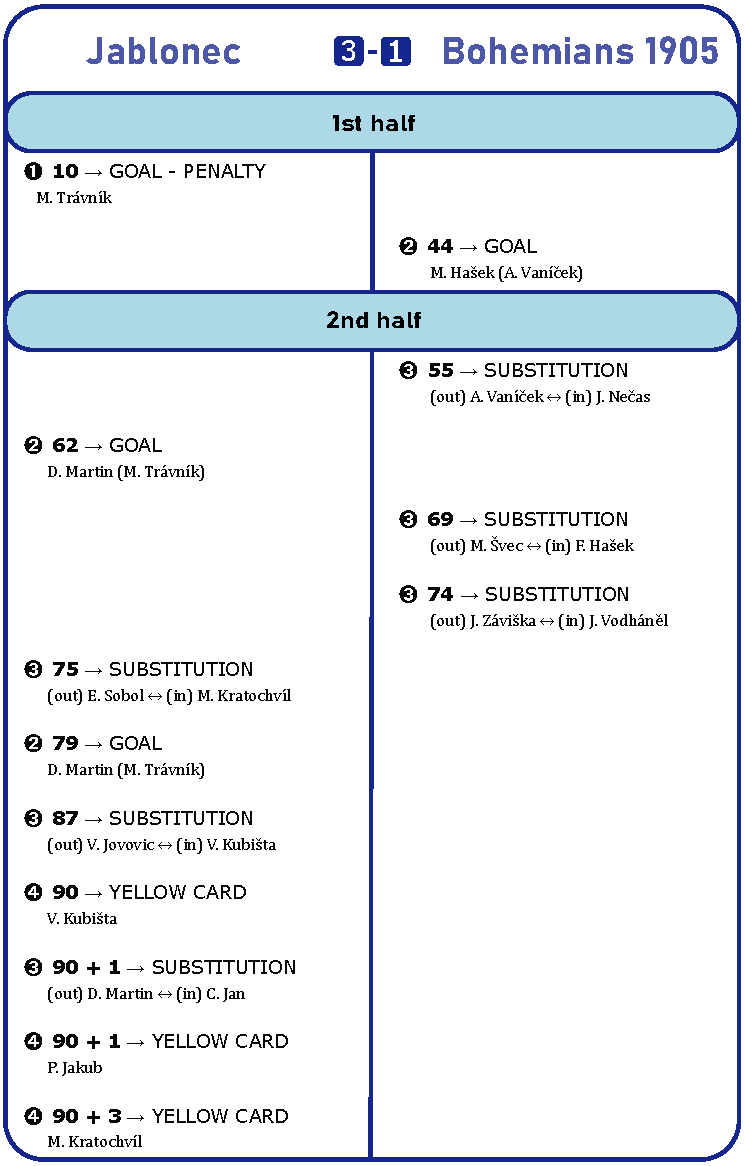
\includegraphics[width=0.9\textwidth]{../img/match_overview.pdf}}
	\caption{Table summary of the example match.}
	\label{fig:overview}
\end{figure}

\section{Structure overview}
The overview of the structure of the solution is shown in \figref{structure}.

Input data with arguments to modify slight functioning (as way of output, or number of texts to generate) are passed to \emph{run.py} (\figref{structure} - 1) (.py will be left out as it is implicit for every module), which is the executable starting point of the program. Parsed arguments are an input for \emph{articles\_generator}, which handles the communication between each module, essentially creating the one-way-pipeline for modules (\figref{structure} - 2, 3, 4, 5) and managing passing the suitable inputs and outputs. Output of this core handler is tuple of strings - title and body of the article.

The \emph{data\_initializer} (\figref{structure} - 2) is as module not present in the original module architecture by \cite{reiter1997building} (described in (TODO-A-odkaz na sekci)). However, since the data is in a raw form, the step of data processing needed to be added to store the data in a more convenient way to further operate with the information given.

Modules (\figref{structure} - 3, 4, 5) correspond to the modular architecture perfectly. \emph{Document\_planner} (\figref{structure}-3) takes data about a match in a convenient inner representation. Creating a \emph{DocumentPlan}, which contains preverbal messages to be said in a sentence. Then these messages are lexicalized in \emph{sentence\_planner} (\figref{structure} - 4) and finally linguistically realised by \emph{linguistic\_realiser} (\figref{structure} - 5). 

Moreover, there are three auxiliary modules to keep the structure of the implementation as clean as possible:
\begin{itemize}
	\item \emph{Data.py}
	\item \emph{Types.py}
	\item \emph{printer.py}
\end{itemize}
These are further described later in (TODO-ref).

\begin{figure}[p]
	\centering{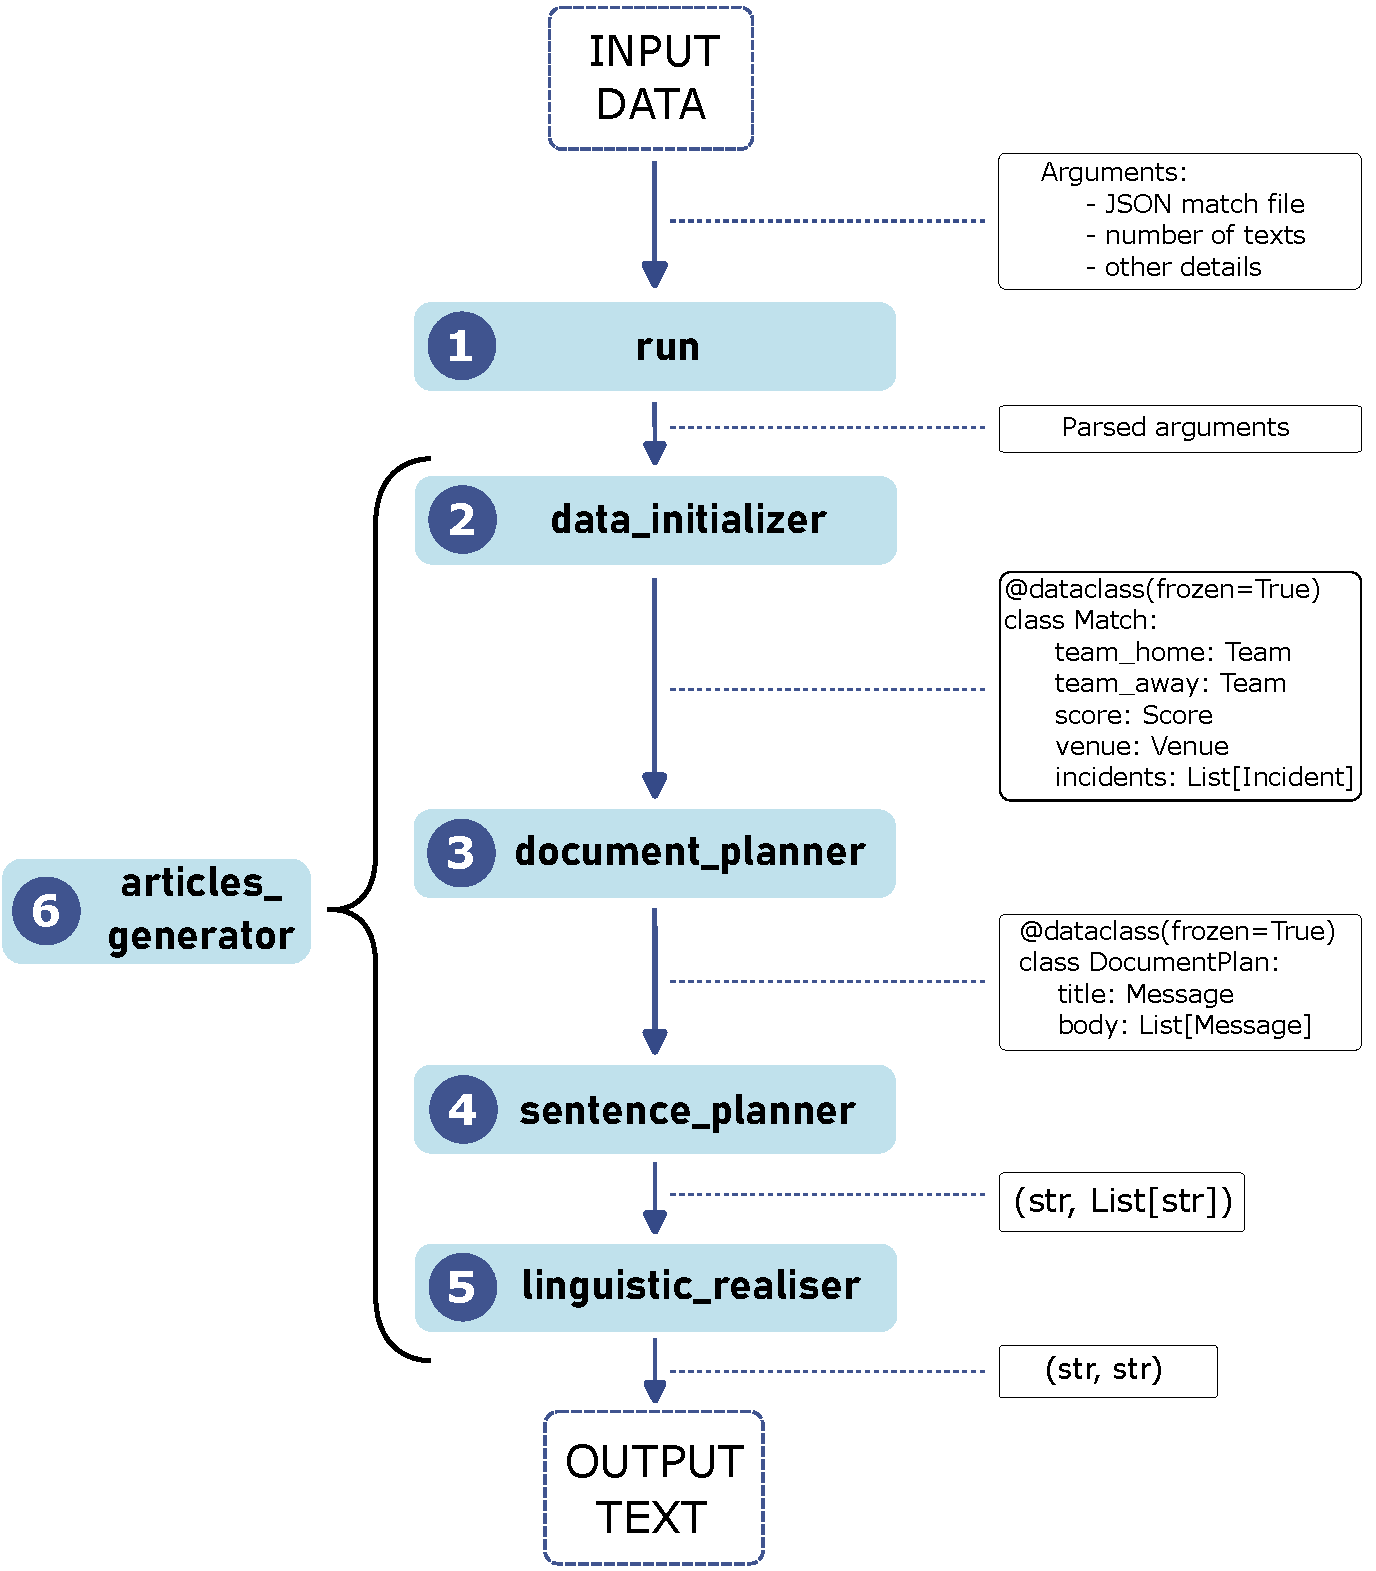
\includegraphics[width=1\textwidth]{../img/program_structure.pdf}}
	\caption{Overview of solution structure.}
	\label{fig:structure}
\end{figure}

\section{Modules implementation}
In this section the implementation of each module is described in detail creating a compact solution in Python. I

\subsection{Auxiliary modules}
\textbf{\textit{Data.py}} groups data classes that store information contained in a JSON file. Namely these entities are \emph{Score, Venue, Country, Player, Team, Time, Incident (+IncidentParent) } and finally the most crucial \emph{Match} that encapsulates each of the class mentioned. Note that these classes are made immutable using \emph{@dataclass(frozen=True)} from package \emph{dataclasses} and then implementing static \emph{create} method. Immutability ensures the data remain intact after manipulating with them frequently in multiple functions across modules. 

Module \textbf{\textit{printer.py}} manages printing different components in a readable way. Since there is a lot of data, even during the development it was more convenient to pretty-print separate results of modules instead of inspecting more nested and complicated states during debugging. Due to numerous alignments and length of string appending separate module was created to not overload other segments of the code.

Lastly, \textbf{\textit{Types.py}} stores enumarate types for different entities. For instance, in module \emph{document\_planner} there is a class \emph{Message} to store attributes of a preverbal message. One of the attribute is type of the message defined as \emph{Types.Message}. This class is implemented in \emph{Types.py} (along with other types, which have arisen so often that separate module was created) as Python's \emph{enumerate()}. Options are \emph{GOAL, PENALTY\_KICK\_MISSED, CARD, SUBSTITUTION, RESULT}. To give one more example, message that reports a card has attribute about type of card stored in \emph{Types.Card} - \emph{YELLOW, RED\_AUTO, RED\_INSTANT} (distinguishing the difference between two yellow cards and instant red card - to highlight the severeness of the foul). Similarly, other types of different-level entities are stored. 

\subsection{Data initializer}
Goal of \textbf{\textit{Data\_initializer}} is to transform data from initial JSON file to more convenient inner representation implemented as system of classes to uphold the principles of object-oriented programming resulting in crisp and well-divided structure.

The implementation is straightforward - we use built-in package \emph{json} to ease the manipulation with a JSON file while initializing classes from module \textbf{\textit{Data}}. 

Two examples of specific records contained in JSON file and their Python representation are shown in \figref{player} and \figref{incident}. 

\begin{figure}[h]
	\centering{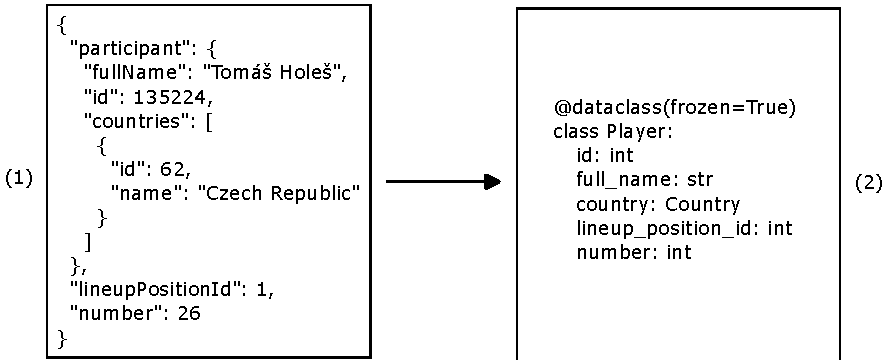
\includegraphics[width=0.9\textwidth]{../img/data_player.pdf}}
	\caption{Transformation of entity \emph{Player} from JSON to a Python class.}
	\label{fig:player}
\end{figure}

Entity {Player} is transformed from its initial JSON representation (\figref{player} - 1) to a easy-to-work-with Python's immutable class \emph{Player} with corresponding attributes. Note that a country has also a proper class \emph{Data.Country}.

\begin{figure}[h]
	\centering{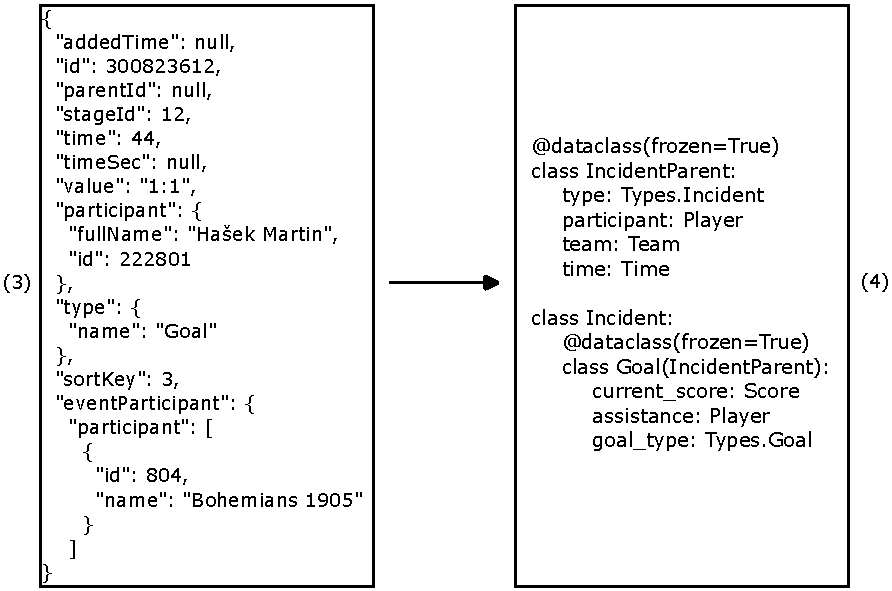
\includegraphics[width=1\textwidth]{../img/data_incident.pdf}}
	\caption{Transformation of entity \emph{Incident} from JSON to a Python class.}
	\label{fig:incident}
\end{figure} 

Entity \emph{Incident} is transformed from JSON (\figref{player} - 3) to a representation as an immutable Python's class (\figref{player} - 4). The class is called \emph{Goal} and it is a subclass of \emph{Incident}. This particular class structure ensures class addressing different types of incidents (goal/card/substitution/penalty kick) as one variable type and therefore enabling the \textit{Data.Match} class to have attribute \textit{incident} storing incidents as \emph{List[Incident]}. Furthermore, every \textit{Incident} subclass also inherits from \emph{IncidentParent} class since these are common attributes for every match incident and it would be inefficient to repeat those attributes multiple times.

Note that this module resolves part of content determination since number of attributes from initial JSON file are not transformed into Python class. For instance starting time of the match was not saved since I personally mark this information as redundant for a article generating. Similarly, more attributes were omitted to avoid useless information. On the other hand, couple attributes end up redundant (e.g. \textit{Country} of \textit{Player}), but these attributes are kept to ensure integrity of the solution and enabling easier further future development. 

\subsection{Document planner}

The aim of this module is to plan the content of the separate messages and their order. Document planner is resolved trivially - each incident is transformed to a separate preverbal message along with fundamental data. 

Implementation is shown in \figref{message} and is similar to Incident structure. Each preverbal message has different arguments and therefore own class. To access messages classes as one variable type there is a system of inheritance, where every message class inherits from \textit{MessageParent} so that they can be distinguished by their according type \textit{Types.Message}. Note that these classes again immutable to ensure data stability.

Unlike message class \textit{Substitution}, which is self-explanatory, classes \textit{Result} and \textit{MissedPenalty} need clarification. 

\textit{Result} message defines the title of the article. The core purpose of the title is to summarise a match in one sentence and hence to report the result/score of the match. 

Content of the \textit{MissedPenalty} is rather obvious, but the reasoning behind the existence of this separate class may not be visible at first glance and relies heavily on domain knowledge. Penalty is a crucial, rare and thrilling event during a football match\footnote{Remember the famous penalty by Antonín Panenka in European Championship finals in 1976 that led to triumph of Czechoslovakia. The kick was groundbreaking and nowadays term 'Panenka' refers to a style of kick, where you only chip the ball in the middle of the net.}. Consequently, every penalty is worth mentioning regardless of the outcome. However, if the penalty is successful the outcome is a goal and we would like to treat the message the same as any other goal. I believe every goal in a football match should be reported since scoring in football is rarer than in other sports in general (compared e.g. to basketball where reporting every basket would be too specific and unnecessary). Contrastingly, the message that reports a missed penalty is not required to be present in the article as this event did not affect the result directly and creates rather a shocking element of the article as players are expected to score from this position. This paragraph further illustrates the hand-crafted principles based on the domain knowledge that are incorporated in the solution.

\begin{figure}[h]
	\centering{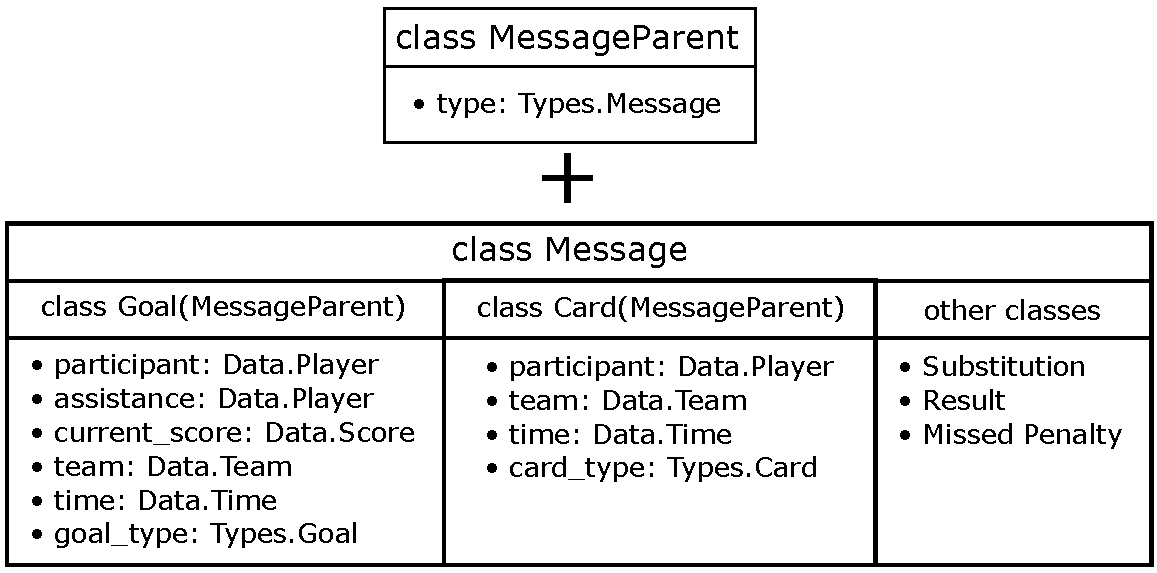
\includegraphics[width=1\textwidth]{../img/message_implementation.pdf}}
	\caption{Implementation of preverbal messages.}
	\label{fig:message}
\end{figure} 

\subsection{Sentence planner}

\subsection{Linguistic realiser}

\subsection{Articles generator}


\section{diskuze řešení - alternativy, rozšíření, další podněty}






















